\begin{frame}[c]
    \frametitle{单片CMOS光学显微光谱仪}
    \begin{columns}
        \begin{column}{.7\textwidth}
            \begin{itemize}
                \item Correia, J.;  De Graaf, G.;  Kong, S.;  Bartek, M.; Wolffenbuttel, R., \textcolor{red}{Single-chip CMOS} optical microspectrometer. Sensors and Actuators A: Physical 2000, 82 (1-3), 191-197.
                \item \textcolor{blue}{重要性:}许多应用,例如通过光学吸收和发射线表征进行化学分析的系统,将受益于低成本单芯片光谱仪的可用性。
                \item \textcolor{blue}{创新点:}结果是芯片可以仅使用四个外部连接来操作,覆盖半高宽 18 nm 的光谱的可见光谱范围。
                \item \textcolor{blue}{意义:}气体和液体成分的识别、光吸收化学分析、发射线表征、比色法和生化分析是微型光谱仪可能有用的一些应用。
                \item \footnotesize{CMOS:互补金属氧化物半导体(Complementary Metal-Oxide-Semiconductor Transistor)}
            \end{itemize}
        \end{column}
        \begin{column}{.3\textwidth}
            \begin{figure}[H] %H为当前位置,!htb为忽略美学标准,htbp为浮动图形
                \centering %图片居中
                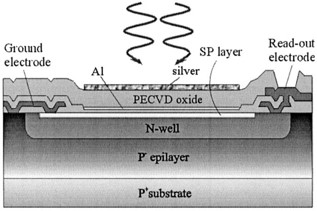
\includegraphics[width=1.\textwidth]{figures/Single-chip CMOS optical microspectrometer_1.jpg} %插入图片,[]中设置图片大小,{}中是图片文件名
            \end{figure}
            \begin{figure}[H] %H为当前位置,!htb为忽略美学标准,htbp为浮动图形
                \centering %图片居中
                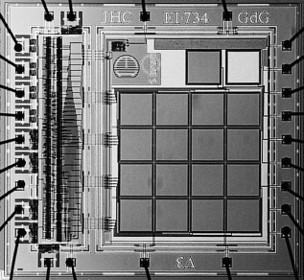
\includegraphics[width=1.\textwidth]{figures/Single-chip CMOS optical microspectrometer_2.jpg} %插入图片,[]中设置图片大小,{}中是图片文件名
            \end{figure}
        \end{column}
    \end{columns}
\end{frame}

\begin{frame}[c]
    \frametitle{单片CMOS光学显微光谱仪}
    \begin{itemize}
        \item 金属 - 介质单腔滤光片
        \item 薄膜结构:45 nm $\mathrm{Ag}$ - (225 $\sim$ 300) nm $\mathrm{SiO_2}$ - 20 nm $\mathrm{Al}$ - $\mathrm{Si}$ 基底
    \end{itemize}
    \begin{figure}[H] %H为当前位置,!htb为忽略美学标准,htbp为浮动图形
        \centering %图片居中
        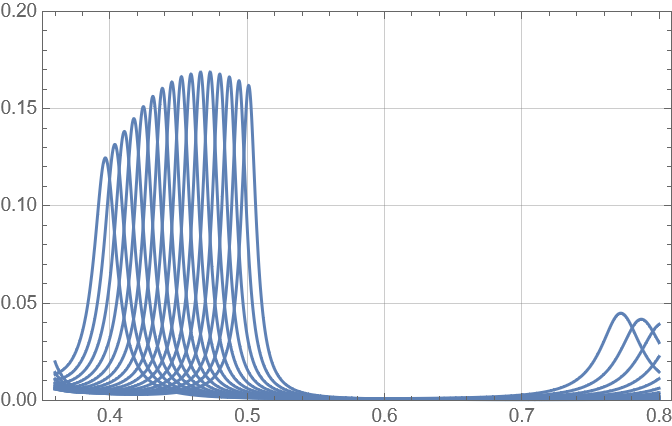
\includegraphics[width=1.\textwidth]{figures/Single-chip CMOS optical microspectrometer_3.png} %插入图片,[]中设置图片大小,{}中是图片文件名
        \caption{透射率与波长的关系} %最终文档中希望显示的图片标题
    \end{figure}
\end{frame}